\section{Project analysis and System requirements}
\phantomsection

\subsection{Problem Definition}
The platform OpenMedia is a rather complex system consisting from several parts. That is why is crucial to break it into smaller modules and logical components that can communicate with each other. There are lots of parts which the application should consist of: data fetching, cleaning the articles and enriching them with proper metadata, interactive modern web application, efficiently storing the data, running tasks independently, communication between system components, how to implement asynchronous messaging between modules, smart visualization of the data, what are the dependencies of some specific technologies, how this dependencies will co-work in combination with the rest of the system. If looked from a bigger scale the problem is not that simple, that's why a deeper level of structured granularity is required.

\subsection{Project Analysis}
The project OpenMedia is a platform used to provide visual models and statistic result based on online media sources from Republic of Moldova. It aims to collect the available articles found on the public sources and use them as a generic source for extracting useful results to be provided to visualization tools. The features offered by OpenMedia will be tools for querying for the desired keywords, in order to construct frequency plots, with options to see to what sources it belongs to. Also it will bring trend detection utilities. By selecting a range of time, it will render the most mentioned terms, and construct bar charts thus communicating the relevance of the popularity.

The platform will consist from two major parts.
\begin{enumerate}
    \item Data gathering platform;
    \begin{itemize}
        \item Fetching the article pages;
        \item Extracting the article;
        \item Storing the article;
        \item Enriching with textual metadata.
    \end{itemize}
    \item Web Client platform.
    \begin{itemize}
        \item A simple and intuitive design;
        \item Launching asynchronous tasks;
        \item Receiving the finished;
        \item Visualization of results.
    \end{itemize}
\end{enumerate}

\subsubsection{Data gathering platform}
This part of the application is focused on gathering data, cleaning and baking it. Simply put, all the heavy lifting of textual data preprocessing is done by this part of the platform. In the figure \ref{data_gathering_mock} is mocked the activity layers of the application. It is important to deliver the data in a format easily operable by the application because the amount of data analysis tricks becomes more various. To be more specific, it is up to client platform to choose the techniques of data consumption. On the one hand it does not sound as an optimized solution but on the other hand it offers flexibility. Data collection is a long and tedious process, that is why it should be better run once. More than that it is advised that all the data changes should be managed in a separate copy. Keeping each stage of data in an immutable state is a wise move. Redundancy is a better choice due to the fact that a project is prone to changes. Running the entire gathering operation from the bottom just in order to add a new feature sounds lethal to a business solution. That is why the OpenMedia platform saves each stage of data.

The articles used by the platform are the public sources of the online media of Republic of Moldova. These are Unimedia, Timpul and Publika. As a future goal is intended to include the other available resources, in order to make the platform more media agnostic. Adding to the system as many resources as possible is a key part of OpenMedia philosophy. The idea is that media sources are usually biased usually by political reasons, meaning that a research in a political area could lead to a less viable result. Beyond that the platform would provide means to deduce predispositions to some governmental parties.

\begin{figure}[!ht]
\centering
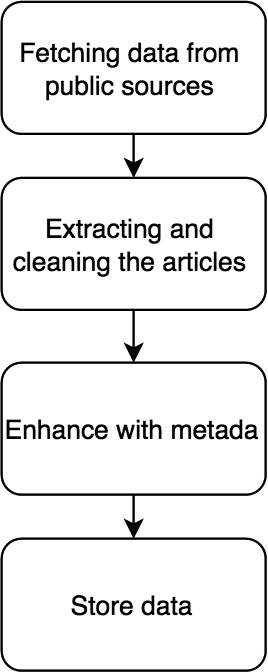
\includegraphics[width=3.8cm]{1_data_gathering}
\caption{Data Gathering platform mockup}\label{data_gathering_mock}
\end{figure}

\subsubsection{Web Client platform}
The client side will represent a web application, a minimalistic layer used for communication between user and the platform. Having a web infrastructure offers the opportunity to make the application easy to access. The only requirement being a modern web browser like Google Chrome, Firefox etc. The focus of the application is to make available the following functionalities.
\clearpage
\begin{itemize}
    \item execute queries on specified words;
    \item execute trend detection queries on specified date rang;
    \item display frequency line charts;
    \item display trends popularity bar charts.
\end{itemize}

This are the basic functionalities provided by the client application. Of course here are also included details such as specifying the media resource, in order to be able to compare the results and extract some useful conclusions from it. The goal is to make the user experience as natural as possible. And due to the fact that he number of functionalities are not so various, creating a natural flow of events will not represent an essential problem. But it should be taken into consideration that a reduced amount of functionalities does not mean a reduced amount of operations. The whole sequence of events is rather complex. It will be described step by step in the next pages of the report.

\begin{figure}[!ht]
\centering
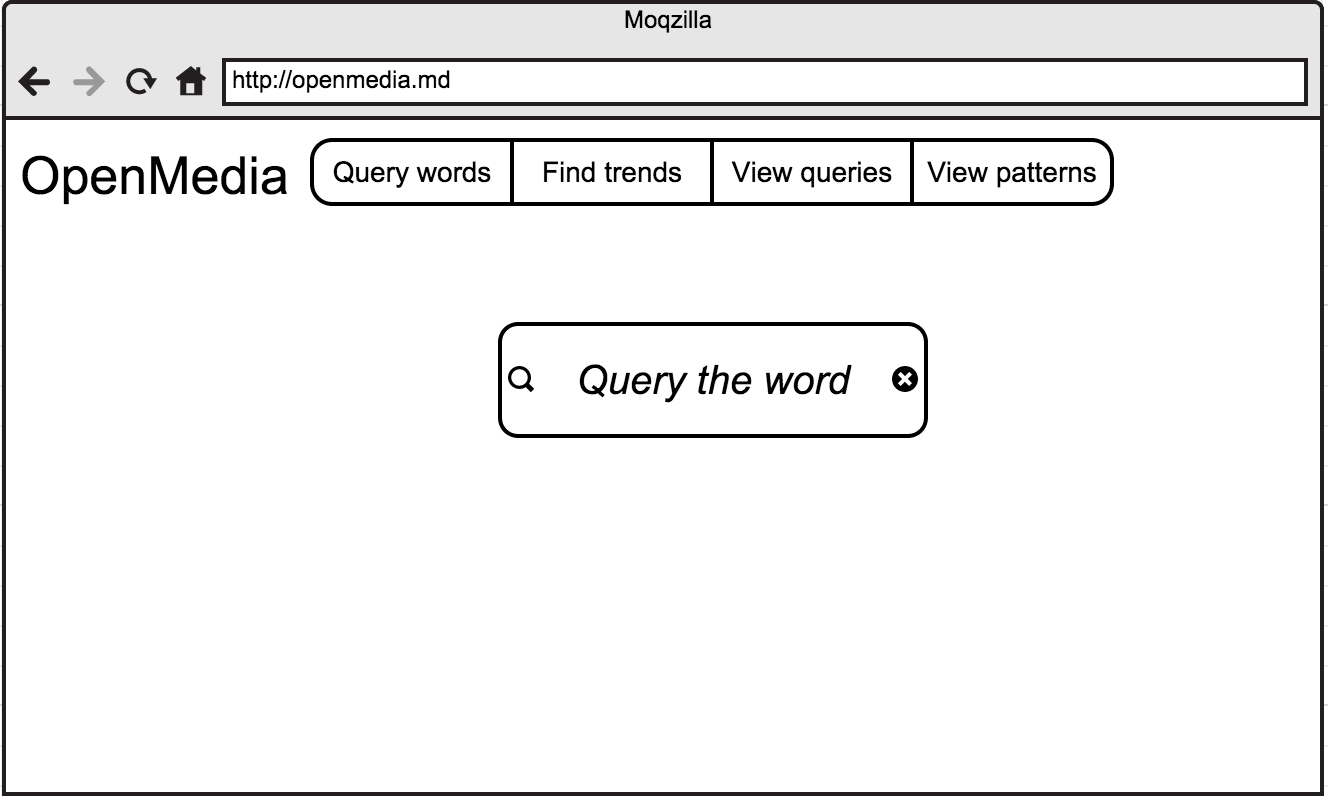
\includegraphics[width=13cm]{1_app_mock_1}
\caption{Primary page view}\label{app_mock_1}
\end{figure}

In order to make an expected view of the application. There are presented some mockups of the web applications. In figure \ref{app_mock_1} is represented the main page. The user has the input box used to execute queries related to word frequency. Because the query execution latency is going to be pretty long, the application is intended to work in an asynchronous way. So after the clicking, a notification will pop up informing that a query was started. Also a pop up notification will be displayed when there are news about the result. After which the result can accessed by clicking on View Queries button. By selecting the specific word, application is transitioning to a result view. The mockup of the page can be observed in figure \ref{1_app_mock_2}. A  plot is rendered representing the intensity per month which the word was mentioned. According to date range, the necessary conclusions be drawn. For example when was the specific word at its peak. When it started to become less popular, what are the spikes, what caused the spikes. This might prove quite valuable information if examined from the right angle. The good part that anyone interested of statistic results can use it. Starting from business entrepreneurs which are trying to research the trendiness of a specific product, a journalist which is interested in popularity of a specific event or entity. The great part about it is that a personal set of queries can be done, thus building a custom aggregation of analytical results

\begin{figure}[!ht]
\centering
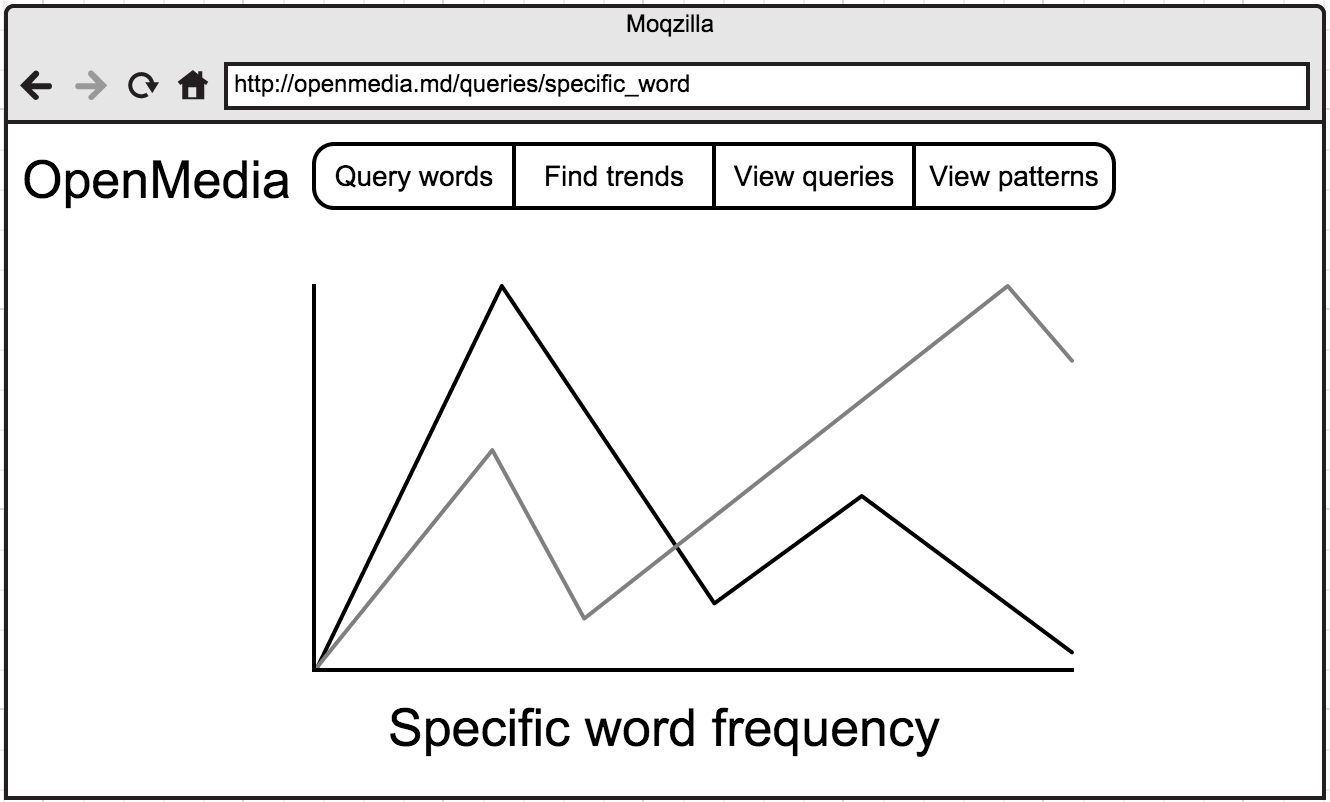
\includegraphics[width=13cm]{1_app_mock_2}
\caption{Frequency plot view}\label{app_mock_2}
\end{figure}

\subsection{Theoretical analysis}
Considering the complexity of the platform, a right amount of research is required in order to construct a workable product. The project OpenMedia consists of two independent separate product. Because both make part of the same new evolving field, data science, the final product represents a usable product which can be used on a local scale. Now will follow a more detailed description of various aspects of the platform, regarding the technologies best suited for building the application, the concepts involved under the hood, means of solving some specific problems.

\subsubsection{Web Sockets}
WebSocket is a protocol providing full-duplex communication channels over a single TCP connection. The WebSocket protocol was standardized by the IETF as RFC 6455 in 2011, and the WebSocket API in Web IDL is being standardized by the W3C.

WebSocket is designed to be implemented in web browsers and web servers, but it can be used by any client or server application. The WebSocket Protocol is an independent TCP-based protocol. Its only relationship to HTTP is that its handshake is interpreted by HTTP servers as an Upgrade request. The WebSocket protocol makes more interaction between a browser and a website possible, facilitating live content and the creation of real-time games. This is made possible by providing a standardized way for the server to send content to the browser without being solicited by the client, and allowing for messages to be passed back and forth while keeping the connection open. In this way a two-way (bi-directional) ongoing conversation can take place between a browser and the server. The communications are done over TCP port number 80, which is of benefit for those environments which block non-web Internet connections using a firewall. Similar two-way browser-server communications have been achieved in non-standardized ways using stop-gap technologies such as Comet.

The WebSocket protocol is currently supported in most major browsers including Google Chrome, Internet Explorer, Firefox, Safari and Opera. WebSocket also requires web applications on the server to support it.

WebSocket reduces latency. For example, unlike polling, WebSocket makes a single request. The server does not need to wait for a request from the client. Similarly, the client can send messages to the server at any time. This single request greatly reduces latency over polling, which sends a request at intervals, regardless of whether messages are available. WebSocket makes real-time communication much more efficient. Polling can always be used (and sometimes even streaming) over HTTP to receive notifications over HTTP. However, WebSocket saves bandwidth, CPU power, and latency. WebSocket is an innovation in performance. It is also is an underlying network protocol that enables to build other standard protocols on top of it. It is also a part of an effort to provide advanced capabilities to HTML5 applications in order to compete with other platforms.

\subsubsection{Data storage}
The whole idea of computer science is wrapped around of ways of manipulating data. From the very start it had issues with finding ways to store data. During the time the hardware evolved and nowadays the disk space does not represent a problem anymore. The actual challenge is how to make interaction with data as efficiently as possible. By interaction is meant means of reading,and querying data. Effectively saving it on the disk, keeping it consistent and avoid data loss. What if data is related to other type of data. How to  implement the relationship between the data. How to make possible reading/writing by multiple users at the same time. This are the actual problems which is confronted in computer science.

The classical solution to this problem are the RDBMS approaches. It is a common choice for the storage of information in new databases used for financial records, manufacturing and logistical information, personnel data, and other applications since the 1980s. Relational databases have often replaced legacy hierarchical databases and network databases because they are easier to understand and use. The relational databases rely on SQL which is a special-purpose language designed for managing data. It is used to query, insert, update and modify data. Because the amounts of data in computer science, until recently, was not so big. Which is why RDBMS were and still are an irreplaceable solutions for managing efficiently relatively small amounts of data. It is because its entire philosophy is built around ACID principle, Atomicity, Consistency, Isolation and Durability. The combination of this 4 principles has granted such a big success to relational databases.

As mentioned above RDBMS is widely used for lots of applications. And successfully solves the given problem and there hasn't been a better alternative on the market. The competition is applied to different implementations of databases, such as PosgreSQL, MySQL, OracleSQL, MsSQL, MariaDB. All of them are quite similar, and each has its strong and weak points. The actual problem appears when the BigData started to get more an more popular. Unfortunately the classical database approach was not enough for the constantly increase of big data demand. Because it enforces a well defined schema, it gets slower and unmanageable when the amount of data is increased.

What developers decided was to loosen up one of the ACID principle and create new brand of database which have a different structure and would allow storing and working with big amounts of data. This is how the term BASE sprang up. Basically Available, Eventually Consistent. Because BASE concept supports the idea of network partitioning, which really means that the database will always have a response disregarding the amount of requests is accessed at the given time. The catch is what kind of response should it have in case of multiple accessing of the database. Two solutions were proposed. First one is that the database should always return a result even though it is not actual and updated. The second solutions is to inform the database user that the service is not available for now. Both solutions have their own applications. Choosing which one to use depends entire on what is better suited for business. The idea of choosing the database model is also presented by CAP theory. CAP states that when choosing a database you can choose only two of the three features. They are Consistency, Availability and network Partition tolerance. In figure \ref{cap} is illustrated in more details the CAP theory.

\begin{figure}[!ht]
\centering
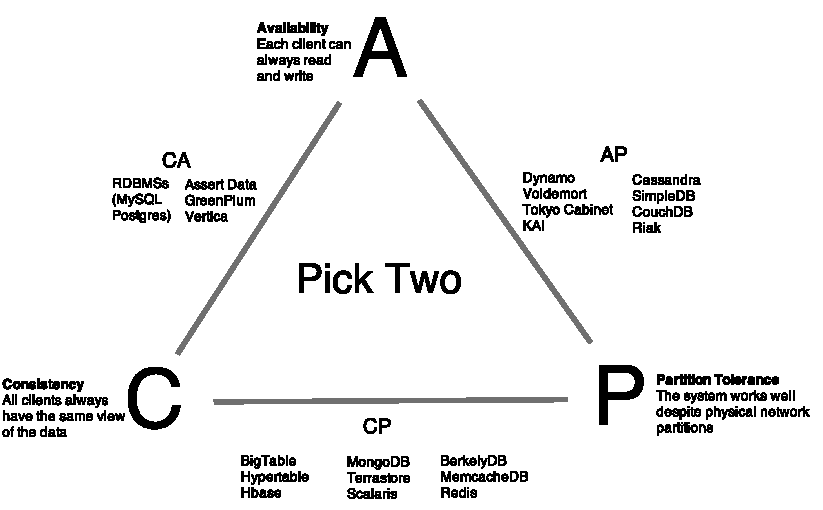
\includegraphics[width=17cm]{1_cap}
\caption{CAP Theory}\label{cap}
\end{figure}

Along with the implementation of conceptual new database the term NoSQL started to spread. The term came from the fact that the new databases were not using SQL for data management. In reality there are more types of conceptual database, and covering all of them under the same umbrella seems too ambiguous.
the most widely used types of databases, not considering RDBMS, are described bellow.

\textbf{Document Based Database} is a new approach of database management. It is used in usual English sense of a group of data that encodes some sort of user-readable information. This contrasts with the value in the key-value store, which is assumed to be opaque data. The basic concept that makes a database document-oriented as opposed to key-value is the idea that the documents include internal structure, or metadata, that the database engine can use to further automate the storage and provide more value.

Document databases contrast strongly with the traditional relational database (RDBMS). Relational databases are strongly typed during database creation, and store repeated data in separate tables that are defined by the programmer. In an RDBMS, every instance of data has the same format as every other, and changing that format is generally difficult. Document databases get their type information from the data itself, normally store all related information together, and allow every instance of data to be different from any other. This makes them more flexible in dealing with change and optional values, maps more easily into program objects, and often reduces database size. This makes them attractive for programming modern web applications, which are subject to continual change in place, and speed of deployment is an important issue. The current most popular implementation of such type of database is MongoDB, CouchDB.

\textbf{Column Based Database} is a database management system that stores data tables as sections of columns of data rather than as rows of data. In comparison, most relational DBMSs store data in rows. This column-oriented DBMS has advantages for data warehouses, customer relationship management systems, and library card catalogs, and other ad hoc inquiry systems where aggregates are computed over large numbers of similar data items.

It is possible to achieve some of the benefits of column-oriented and row-oriented organization with any DBMSs. Denoting one as column-oriented refers to both the ease of expression of a column-oriented structure and the focus on optimizations for column-oriented workloads. This approach is in contrast to row-oriented or row store databases and with correlation databases, which use a value-based storage structure \cite{wiki_column_based_db}. Such type of database implementations are BigTable, Casandra, DynamoDB.

\textbf{Key Value Database} use the associative array (also known as a map or dictionary) as their fundamental data model. In this model, data is represented as a collection of key-value pairs, such that each possible key appears at most once in the collection.

The key-value model is one of the simplest non-trivial data models, and richer data models are often implemented on top of it. The key-value model can be extended to an ordered model that maintains keys in lexicographic order. This extension is powerful, in that it can efficiently process key ranges. Example of such type of database implementations are Redis, Memcache, Voldemort.

\subsubsection{Data Visualization}
Human has a long history with basic data visualization, and data visualization is still a hot topic today. The history of visualization was shaped to some extent by available technology and by the pressing needs of the time, they include: primitive paintings on clays, maps on walls, photographs, table of numbers, these are all some kind of data visualization, although nowadays this kind of art may not be called data representation. Visualization is the graphical presentation of information, with the goal of providing the viewer with a qualitative understanding of the information contents. It is also the process of transforming objects, concepts, and numbers into a form that is visible to the human eyes.

Big data is creating unprecedented opportunities for businesses to achieve deeper, faster insights that can strengthen decision making, improve the customer experience, and accelerate the pace of innovation. But today, most big data yields neither meaning nor value. Businesses are so overwhelmed by the amount and variety of data that they struggle just to store the data, much less analyze, interpret, and present it in meaningful ways.

The trend toward visualization based data discovery tools is worth exploring by any business that seeks to derive more value from big data. The potential business benefits are immense, and data governance best practices can be used to help ensure a safe transition. As demonstrated by three usage examples from TIBCO Software, the world’s second largest data discovery vendor, real world applications of visualization based data discovery tools are already delivering greater customer and market insights to businesses around the world.

Data analytics and visualization are not new. For decades, businesses have collected data, analyzed it using a variety of BI tools, and generated reports. Businesses are finding that this traditional reporting process does not work nearly as well for big data, and certainly is not sufficient to capture the potential value that big data represents. The primary challenges stem from what are commonly termed the “three Vs” of big data: volume, variety, and velocity. Most traditional reporting and data mining tools cannot handle the vast volume of big data, although the variety and velocity of the data often present even greater challenges.

Data can be represented in various way, it can have as many forms as a human brain can imagine. Even so there are already steady classical patterns for data visualization which are well known by common humans, and more important it is easy to read.

\begin{description}
    \item Simple bar charts are the most common form of data visualizations. Typically they only display different quantities of single variable data. However other variations, such as stacked bar charts or multi set bar charts can be used to compare multiple variables using bars;

    \item Line graphs are created by plotting points on a Cartesian grid, usually with the horizontal axis representing time. They are very powerful because without looking at the specific data, they show how a variable develops over time (from left to right);

    \item Stacked area charts are similar to line charts, however with the added value of filled areas. The data that is stacked adds up to a total of all variables combined. For example a business might use stacked area charts to visualize their total income, with each stacked area a different income channel;

    \item Pie charts are the most common visual used to compare proportional data. They give viewers a very quick understanding of the distribution of the data. Pie charts are not useful when comparing many pieces of data with relatively close values;


    \item Ring charts are used to visualize the distribution of a data set. The advantage is they compare similar data sets. The alternative would be to place multiple pie charts next to each other, this can also be viewed as a space-saver;

    \item Scatterplots are created by plotting independent points on a Cartesian grid. Scatter plots are often used to find the relationship between data or to reveal information such as trends within the data which are not easily visible when in a table. Only works with two dimensional data;

    \item Bubble charts display more dimensions of data by varying size (or also color, texture, etc) of the bubbles. It therefore can display multiple dimensions of data in a two dimensional display;

    \item Tree diagrams are often used when wanting to represent the strict hierarchy of data. They are most often used to represent strict hierarchies such as family trees or how data is stored in a computer system;

    \item Diagram maps visualizations are used to primarily represent the connections between different nodes or points. Their purpose is to show which points are connected to each other. Common examples of diagram maps are metro maps and social network visualizations;

    \item Maps are used when the data is related to a specific location (for example a city, or country). The advantage is that their spatial representation directly relates to a real world situation. However at times can be difficult to read.
\end{description}

\subsubsection{Modern Web Application}
Web applications are heavily using HTTP protocol as means of transporting the data. The thing is that HTTP is a stateless protocol. For every request made by a client a TCP socket is opened. The HTTP server is receiving the request and handled by the application layer which does the response decision. When the response is sent back to the client, the TCP socket is closed and the transaction ends. The whole chain of events is repeated basically at every user interaction. In the result the web application is becoming a stateless application itself. At least that was valid until concept of Web 2.0 was introduced in 2004. Java Script started to become more popular because it gave the power to animate the pages and create a more humane UX. But the magic was behind the AJAX technology. The concept introduced by AJAX was making a web page run asynchronous requests and make live partially DOM changes. Developers could create web applications which did not require full page reload at while interacting with the page. Successfully implementation of this concepts are Facebook, Gmail, Twitter etc. AJAX, JQuery and other Java Script technologies brought web applications one step closer to the desktop applications experience.

What is targeted now are the single page applications. The main reason is that they are able to offer more native application like experience to the user. This is hard to do with other approaches. Supporting rich interactions with multiple components on a page means that those components have many more intermediate states. Server side rendering is hard to implement for all the intermediate states. Small view states do not map well to URLs.

Single page applications are distinguished by their ability to redraw any part of the UI without requiring a server round trip to retrieve HTML. This is achieved by separating the data from the presentation of data by having a model layer that handles data and a view layer that reads from the models. Interaction with the single page application often involves dynamic communication with the web server behind the scenes.

Here are enumerated a set of popular technologies which offers the possibility of building single page applications:
\begin{itemize}
    \item Ember;
    \item Angular;
    \item React (recently introduced by facebook);
    \item Meteor;
    \item Marionette.
\end{itemize}
All this frameworks are built using Java Script languages, meaning that this is the right language for building modern web UX. Especially when so many communities were present which are eager to make the tools better, more easy to easy and scalable.

Due to the fact that single page applications are highly functions, they also include a complex architecture. For instance in figure \ref{ember_architecture} is the conceptual structure of Embre JS framework. It is pretty hard to wrap the head around the structure, but once there is a basic understanding of the logical layers, building applications becomes joy for a developer.

\begin{figure}[!ht]
\centering
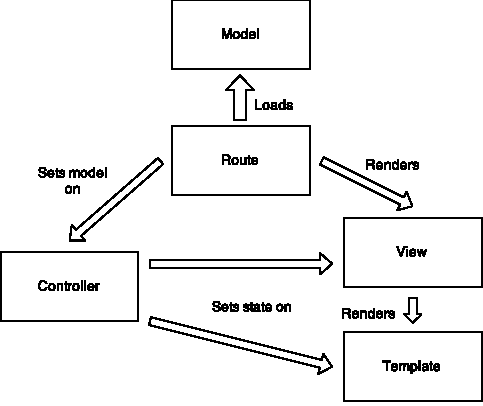
\includegraphics[width=10cm]{1_ember_architecture}
\caption{Ember framework architecture}\label{ember_architecture}
\end{figure}

Until now everything discussed was related to building the front part of a modern web application. But a web application consist also from the backed part. The HTTP application which listens client requests. For building one there are a lot of frameworks which easily allows to scaffold a prototype. MVC based frameworks are powerful and provides lots of functionalities out of the box. And the good thing is that the majority of frameworks are mature and stable. Here are a list of frequently used solutions:
\begin{itemize}
    \item Ruby on Rails;
    \item Django;
    \item Spring;
    \item ASP .NET;
    \item Symphony.
\end{itemize}
The thing is that the mentioned technologies have huge stacks which sometimes are not needed when building a smaller application, or scalable one. Besides for building modern web applications where the client application is developed in a Java Script framework, means that the "V" (view) part from MVC is not needed anymore. Plus there are already on the market lightweight web technologies such as Sinatra, Flask, Node (in combination with express library). This type of application can serve just as good. In case if new module is required by the application, it can be easily added to the micro-framework stack. In ruby this is done by using gemfiles (gems are libraries in Ruby language) were gems can be easily added and installed effortlessly.

\subsubsection{Data Journalism}
According to wikipedia, Data journalism is a journalism specialty reflecting the increased role that numerical data is used in the production and distribution of information in the digital era. It reflects the increased interaction between content producers (journalist) and several other fields such as design, computer science and statistics. From the point of view of journalists, it represents "an overlapping set of competencies drawn from disparate fields". \cite{wiki_data_journalism}

The journalists main resource for their work is data, and it was so from the very begging of the journalism. The computer revolution from the 20th century revealed massive opportunities for an a lot of economical fields (and not only). Journalism started integrating data by bringing computer technologies into their daily lives. The nowadays explosion of technologies such as Internet, cloud computing, high performance of mobile devices, easy accessible open source software influenced a lot the modern journalism leading to emergence of data journalism. This new term represents a new extended branch of traditional journalism by involving more data in the field. Decades after early pioneers successfully applied computer-assisted reporting and social science to investigative journalism, journalists are creating news apps and interactive features that help people understand data, explore it, and act upon the insights derived from it. New business models are emerging in which data is a raw material for profit, impact, and insight, co-created with an audience that was formerly reduced to passive consumption.

Journalists around the world now are faced with exciting challenges of writing reports and stories based on deductions made on vast amount of data which is daily increasing and changing. The data generation source are diverse, network lives, businesses, government, politicians, popularities etc. While the potential of data journalism is immense, the pitfalls and challenges to its adoption throughout the media are similarly significant. Global threats to press freedom, digital security, and limited access to data create difficult working conditions for journalists in many countries. A combination of peer-to-peer learning, mentorship, online training, open data initiatives, and new programs at journalism schools rising to the challenge, however, offer reasons to be optimistic about more journalists learning to treat data as a source.

Data visualization is an entire field which is developing alongside data growth. While the tools for visualization are interesting and fancy, visual results alone does not represent much value. It is the story and conclusions which can be drawn from the visual tools what actually matter. A good analogy is the bread preparation, the whole chain of events, starting from sowing the seeds and ending with backing the bread. The story represents the bread in this cycle, the final result, the product which can be published and consumed.The embrace of open source software and agile development practices, coupled with a growing open data movement, have breathed new life into traditional computer-assisted reporting. Collaboration across newsrooms and a focus on publishing data and code that show your work differentiate the best of today’s data journalism from the CAR of decades ago.

Data journalism can be created quickly or slowly, over weeks, months, or years. Either way, journalists still have to confirm their sources, whether they are people or data sets, and present them in context. Using data as a source would not eliminate the need for fact-checking, adding context, or reporting that confirms the ground truth. Just the opposite, in fact. Around the world, a growing number of data journalists are doing much more than publishing data visualizations or interactive maps. They are using these tools to find corruption and hold the powerful to account. The most talented members of this journalism are engaged in multiyear investigations that look for evidence that supports or disproves the most fundamental question journalists can ask: Why is something happening? What can data, related to narrative structure and expert human knowledge, tell about the way the world is changing?

In the hands of the most advanced practitioners, data journalism is a powerful tool that integrates computer science, statistics, and decades of learning from the social sciences in making sense of huge databases. At that level, data journalists write algorithms to look for trends and map the relationships of influence, power, or sources. As they find patterns in the data, journalists can compare the signals and trends they discover to the shoe-leather reporting and expert sources that investigative journalists have been using for many decades, adding critical thinking and context as they go. In addition to asking hard questions of people, journalists can now interrogate data as a source.

\subsubsection{Web services}
Building complex systems is not a simple task to do and usually they consist of smaller logical parts which communicates trough interfaces. A modern distributed application usually runs on different machines. This is a wise choice to do, for multiple reasons. One is the easiness to troubleshoot problems. But with great power comes great responsibilities. On one hand it might prove quite difficult and expensive to run instances of different applications to run the system, on the other hand it can scale efficiently with the increasing demand. One more case might be to build an application which integrates many other public available services and APIs. In the end the point is that the applications should be able to communicate efficiently over the web. Various software are built in different programming languages, are running on diverse operating systems, hence a transparent communication model is needed which is language agnostic. That is how the web services protocols came to existence. During the time they have evolved into a set of communication standards which offered developers the opportunity to construct decoupled systems. The more decoupled the application is, the more testable and maintainable it is.

In order to define the standards, a set of rules are needed to be defined, such as:
\begin{itemize}
    \item How can a software perform a request to another system;
    \item What is the set of parameters should be set in the request;
    \item What should be format of the request;
    \item What are the logical parts from which the request consists;
    \item How should the response be represented;
    \item How should the errors be described.
\end{itemize}

As a result, on the market persist two approaches of constructing web services, SOAP and REST. Each approach have their strong points and weaknesses and both heavily relies on HTTP protocol, in case of SOAP it also supports other transport protocols.

\textbf{SOAP} is a messaging protocol which have the entire architecture wrapped around XML data representation. In a nutshell, it is a method of communication between two applications. An example of SOAP communication is represented in figure \ref{soap} The protocol specifies how exactly the HTTP headers should be encoded. A SOAP provider comes in hand with a WSDL file which represents the description of the web service. Things like the possible parameters and their formats, the structure of the message, what is the response format, how it can be correctly accessed. The communication via SOAP protocol is also done using an XML formated files. The structure of the the request and response is documented in the WSDL file and it is validated with the help of XSD schema.

\begin{figure}[!ht]
\centering
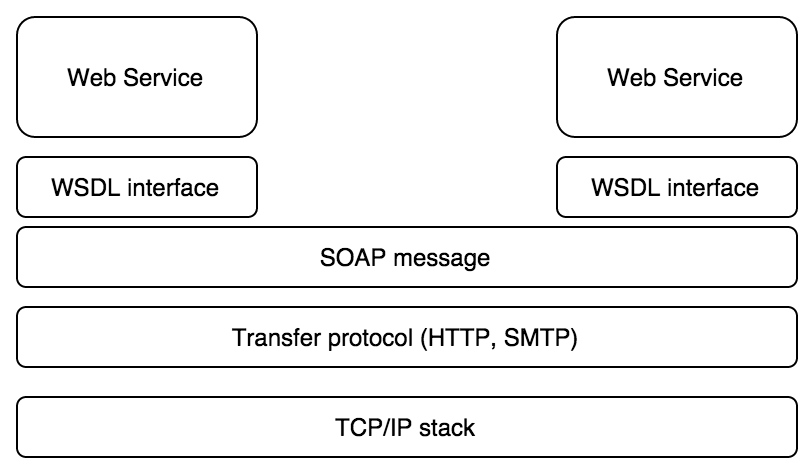
\includegraphics[width=11.5cm]{1_soap}
\caption{An example of SOAP communication}\label{soap}
\end{figure}


SOAP represents the next evolving stage between computer communication at he application layer. It was able to replace RPC technologies such as DCOM, CORBA, Java RMI. This reinstatement was highly needed because RPC technologies were brining a complex coupling to the programming language, which might prove a bad thing, as long as a panacea type programming language does not exist. On the other hand the SOAP calls are much slower comparing to native RPC applications. There tends to be firewall latency due to the fact that the firewall is analyzing the HTTP transport. SOAP calls are much more likely to get through firewall servers, since HTTP is typically Port 80 compliant, where other calls may be blocked for security reasons. Since HTTP requests are usually allowed through firewalls, programs using SOAP to communicate can be sure that the program can communicate with programs anywhere. SOAP is focuses on exposing pieces of application logic (not data) as services, platform operations. It aims for accessing named operations, each implement some business logic through different interfaces. An advantage offered by SOAP is the WS-Security which adds some enterprise security features. Supports identity through intermediaries, not just point to point (SSL). It also provides a standard implementation of data integrity and data privacy.

\textbf{REST} is a simple stateless architecture that generally runs over HTTPS/TLS.This type of web service focuses on a reduced and very well defined amount of operations. The most common operations provided by a REST platform are CRUD. The flexibility is given by assigning resources their URI. The neat part is that it heavily relies on URLs. The REST philosophy is deeply entangled with HTTP protocol implementation, for instance the HTTP verbs GET, POST, PUT, DELETE, PATCH etc, are a part of REST RFC. Although it is just a set of guidelines and best practice, if implemented correctly the application avoids ambiguity. This is a blessing and a curse at the same time. Due to the fact that REST RFC is not a set of rigid requirement, developers tend to misinterpret the usage of some methods method. And example is overusing the "POST" method. Hence a lot of debates, discussions and even holly wars are held on this topic. The good part is that it doesn't need tedious descriptor files such as WSDL in order to describe a REST application. The documentation is usually done in textual manner, just like code documentation. REST gained a lot of popularity as being a simpler alternative to SOAP and WSDL-based web services. And the most viable example is the implementation of the entire Word Wide Web. One strong thing wielded by REST applications is that the message and response content can be delivered in any type of format. The most used are XML based format such as HTML, and for API platforms JSON is the most common and handy format, and it has lots of advantages against XML, such as readability, payload size, easy integrable with dynamic languages, it is data oriented.

Nowadays JSON is becoming the preferred format especially for RESTful APIs. Because of the format simplicity sometimes it gets harder to define the communication structure. Which is why JSON community is working now on an elegant format called JSON-api. It simplifies a lot things in terms of message structure. It resembles to WSDL only it is less restrictive and more intuitive. Another alternative for structuring the message format is HATEOAS. The purpose it aims is defining application state using hypertext.

\subsubsection{Hadoop Mapreduce}
In the last 10 years terms like Big Data, NoSQL, Hadoop, Mapreduce were so frequently discussed that some of them became bloated. For instance, what is Big Data? how "Big" is the data? In 2003 Google released a paper about Google File System, and later in 2004 a Mapreduce paper. Being a company which works with indeed extremely big data, sizes in terms of petabytes and more, they have started to search for solutions how to manage such amounts. And due to the fact that the computational power was getting cheaper by day, they have come up the idea of building file systems which would be able to run on computer clusters. In the path of finding the methods to operate with the huge amounts of data they have seen that the traditional RDBMS database engines would not fit their requirements, so they've came up with an alternative. On 2004 they started working on a new kind of data base based on a different concept, BigTable. A database which exchanges the classical ACID rules with scalability, availability and other positive aspects which would solve their problem. Of course Google is not the only company working with huge amounts of data, resulting in other technologies which were developed based on similar concepts. For instance Amazon came up with DynamoDB, a database which works on the same principle as BigTable, instead it was focused on offering availability instead of consistency (a customer should always be able to buy even though the product is not present in stock). Another example is Yahoo, who came up with Apache Hadoop, a great technology released under the Apache open source license. It is a files system which can work on multiple computers and indeed successfully solve the problem of processing big amounts of data.

After the successful stories of the leading companies, the terms Hadoop, BigData, NoSQl, started to become popular and spread like a fever. Of course lots of companies started using this technologies, because you have to follow the cool kids. The problem was that companies, especially new one, were not making the business smart decisions when choosing the technologies. For instance building an application using a schemaless database. After making the wrong decision it was realized that the application structure actually needed schema. It resulted in managing schema consistency by the application layer, which is an additional layer of complexity that can be handled by a traditional RDBMS engine. A analogous story is related by the Olery company \cite{mongo_to_postgres}. Many startups started to use the newly discussed solutions, forming communities, thus the deceiving labeling started. Everything which is not RDBMS is NoSQL, a term which was intended to be used as a twitter hashtag now covers under its umbrella all the databases which does not rely solely on ACID principles. The same situation is with Big Data. What is the actual size of the data required for being called "big". There are lots of speculations on this topic.

\textbf{Hadoop} is a framework used for distributed storage and distributed processing of large scale of data sets. It can benefit from cheap computation power by running on a mediocre computer cluster. The platform is designed by taking into consideration the hardware failure. It is natural that at some point in time a machine from the cluster will stop running. Hadoop embraced this problem and solved it at the software level. Although Hadoop is best known for MapReduce and its distributed filesystem (HDFS, renamed from NDFS), the term is also used for a family of related projects that fall under the umbrella of infrastructure for distributed computing and large-scale data processing. As the Hadoop ecosystem grows, more projects are appearing, not necessarily hosted at Apache, which provide complementary services to Hadoop, or build on the core to add higher-level abstractions.

Applications that run on HDFS have large data sets. A typical file in HDFS is gigabytes to terabytes in size. Thus, HDFS is tuned to support large files. It should provide high aggregate data bandwidth and scale to hundreds of nodes in a single cluster. It should support tens of millions of files in a single instance.

HDFS has a master/slave architecture. An HDFS cluster consists of a single NameNode, a master server that manages the file system namespace and regulates access to files by clients. In addition, there are a number of DataNodes, usually one per node in the cluster, which manage storage attached to the nodes that they run on. HDFS exposes a file system namespace and allows user data to be stored in files. Internally, a file is split into one or more blocks and these blocks are stored in a set of DataNodes. The NameNode executes file system namespace operations like opening, closing, and renaming files and directories. It also determines the mapping of blocks to DataNodes. The DataNodes are responsible for serving read and write requests from the file system’s clients. The DataNodes also perform block creation, deletion, and replication upon instruction from the NameNode. In figure \ref{hadoop_architecture} is represented the HDFS architecture.

\begin{figure}[!ht]
\centering
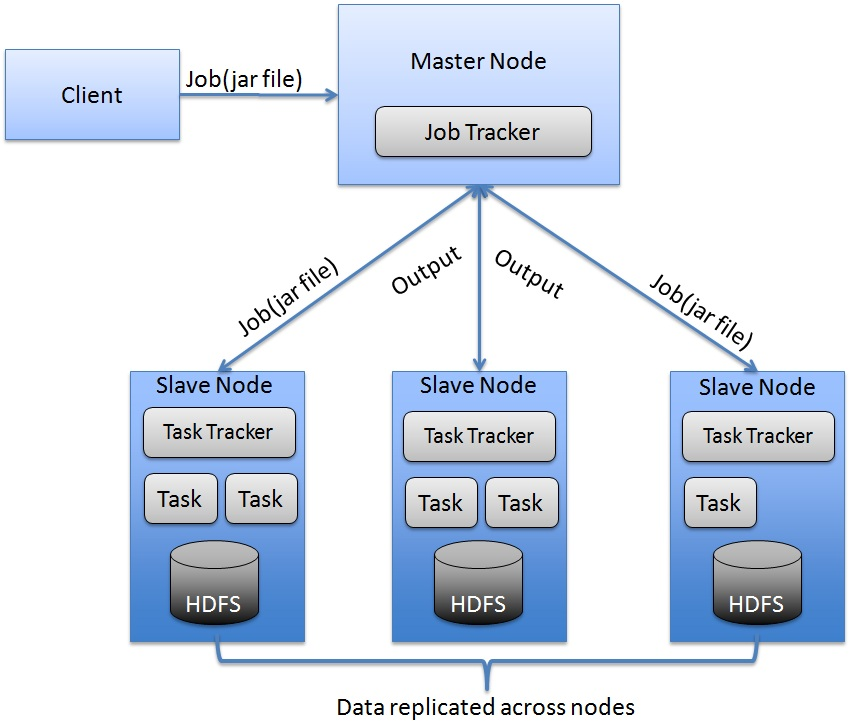
\includegraphics[width=13cm]{1_hadoop_architecture}
\caption{Hadoop architecture \cite{data_mining_image}}\label{hadoop_architecture}
\end{figure}

The NameNode and DataNode are pieces of software designed to run on commodity machines. These machines typically run a GNU/Linux operating system (OS). HDFS is built using the Java language; any machine that supports Java can run the NameNode or the DataNode software. Usage of the highly portable Java language means that HDFS can be deployed on a wide range of machines. A typical deployment has a dedicated machine that runs only the NameNode software. Each of the other machines in the cluster runs one instance of the DataNode software. The architecture does not preclude running multiple DataNodes on the same machine but in a real deployment that is rarely the case.

\textbf{Mapreduce} is a rather primitive operation. It has a brute-force like approach. It is a batch query processor, and the ability to run a query against an entire dataset and get a result in reasonable amount of time is an astonishing thing. It opens an entire new perspective of processing data. The algorithm works in the following way. The user specify a map function which is applied to every record. The goal is to emit a key value pair to generate a set of intermediate key/value pares. The reduce function merges all intermediate values associated with the same intermediate key. Many real problems can be modeled under this concept. Programs written in this functional style are automatically parallelized and executed on a large cluster of commodity machines. The run-time system takes care of the details of partitioning the input data, scheduling the program's execution across a set of machines, handling machine failures, and managing the required inter-machine communication. This allows programmers without any experience with parallel and distributed systems to easily utilize the resources of a large distributed system. Here is an example of map reduce executed in MongoDB \ref{mongo_example}. MongoDB API involves a native mapreduce feature.

\lstinputlisting[language=Java, caption={Mapreduce example in MongoDB}, label=mongo_example]{../src/map_reduce_example.js}

\subsubsection{Lexical analysis}
Open Media project works with articles fetched from the available public sources. As data value it represent just massive chunks of text. Working with plain text might prove a problematic. The reasons are that a spoken language such as English or Romanian (in this particular case) are vast and complex. More than that they might prove to be ambiguous. A simple task like determining the part of speech of a specific word might prove a complex action. The same word might have different meanings in different circumstances. Which is why a probabilist model based on machine learning has to be constructed in order to detect word's context and determine the part of speech it belongs to. Having a text enriched with metadata such as a part of speech is proved to be useful for advanced text analysis. A trivial case is for eliminating the stop words. There are different approaches for this problem. First one is having a dictionary with stop words and check every word if it is a part of the record. The second approach is to assume that all the stop words have a length lesser than for. The issue with this is that there are a lot of exception thus not feasible to fit cluster the words solely on number of characters. The approach which will have an acceptable error rate and will work quite fast (in comparison with a dictionary check) would be, first to detect the part of speech, followed by words elimination which refers to the stop word part of speech.

The process described above is one of the many kinds of text preprocessing tasks which involves lexical analysis. Many of theses processes work hand in hand with another. Usually one can operate on a dataset which is a result of the previous one. Here are listed one of the operations regarding lexical analysis:
\begin{itemize}
    \item Tokenization;
    \item Part of speech tagging;
    \item Lemmatisation;
    \item Text Segmentation;
    \item Chunker;
    \item Syllabification;
    \item Stemming.
\end{itemize}

\textbf{Natural Language Processing} is a field of computer science, artificial intelligence and computational linguistics which studies the interactions between computers and human languages. One of the main challenge of this field involves natural language understanding, where computers are able to extract meaning out of human language input. The classic approach of solving this problem was by hand coding a big set of rules which the machine has to follow. In such way decision trees models were created, basically a lots of "if else" statements. But unfortunately a natural language is a rather complex concepts, and catching all ambiguities makes the decision tree unmaintainable. In the end the traditional decision trees usually resulted in a rather primitive solution. Modern NLP uses lots of machine learning algorithms under the hood. The idea is to apply the learning on a set of corpora where a corpus is a set of documents, sentences which have been hand-annotated with the correct values to be learned. The annotations representing metadata such as part of speech, the word root, synonyms etc. Having a probabilistic model gives the advantage that in a specific situation the solutions can be multiples, with different chances. Usually such type of results are better suited as being a part from a larger system.

\textbf{Tokenization} is a part of NLP field. The first being the tokenization. It represents the process of breaking a string into words, symbols, phrases or other meaningful elements which could be called tokens. Typically the segmentation is done at the word level. The traditional implementation relies on simple heuristics. Tokens are usually separated by whitespace or punctuation characters. Most of Latin alphabet based languages use inter-word spaces (eg New York-based). For such kind of languages the solutions is straightforward. The grade of complexity is much more increased for languages written in scriptio continua such as Ancient Greek, Chinese, Thai.

\textbf{Lemmatization} is another important part of NLP. The idea behind it is to reduce the word to a canonical form. Similar words, or with the same root would have the same result after passing the lemmatisation process. This will give the opportunity to operate with a group of words from the perspective of a single entity. The stemming process is rather similar. The difference is that stemming can be applied to an independent word, while lemmatization works based on the word context, meaning that it has a more complex algorithm on the background. The process already requires additional metadata such as the part of speech of the word. Even though the stemming algorithm is more primitive, due to the fact that it doesn't discriminate the word meaning, the implementation algorithm is much simpler. This fact gives an upper hand for a data analysis process, especially when the computational speed is the bottleneck. An example of lemmatization is that the algorithm ensures that "traveling", "traveled" will be recognized as the same word "travel". This aspect is crucial in context of OpenMedia, if the words are not brought to a canonical form, then the frequency analysis would have an increased error rate, which would lead to an unreliable platform not likely to be used by users.

\subsubsection{Data Mining}
According to wikipedia sources, data mining, an interdisciplinary subfield of computer science, is the computational process of discovering patterns in large data sets involving methods at the intersection of artificial intelligence, machine learning, statistics, and database systems. The overall goal of the data mining process is to extract information from a data set and transform it into an understandable structure for further use. \cite{wiki_data_mining}

\begin{figure}[!ht]
\centering
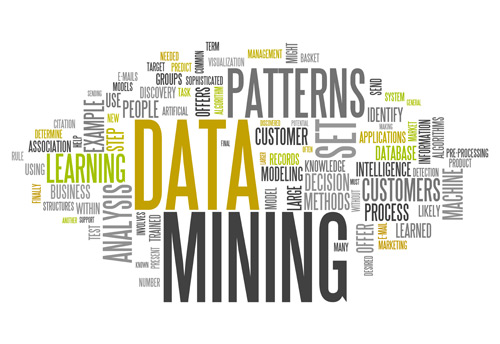
\includegraphics[width=9cm]{1_data_mining}
\caption{Data Mining}\label{data_mining}
\end{figure}

The purpose of data mining is to conduct automatic or semi-automatic inquiries on large amounts of data in order to extract patterns such as groups of records, unusual data, dependencies. In order to perform operations of this scale usually special database techniques are needed. One of are them spacial indexes. This kind of indexed is created based on geospatial data structure, and it helps to increase the performance for queries such as finding the distance between two places. The kinds of patterns detected in a data mining task can be use for further analysis, machine learning, events prediction. Twitter introduced a curious research, based solely on people tweets they have created an influenza pandemic prediction model. It is astonishing that a platform used for posting short textual messages was used for predicting a biological phenomenon. What if the research is done on a dataset strictly target to the analyzed field. Another successful data mining research was done for exploring some specific cancer drugs. Before the research, the result was that the drug (eg X) was working in the 20\% of cases. After the genetic research, it was found out the patient's genetic configuration of successful cases. Now it was possible to identify the people to whom the drug X will work for 100\%. The examples described above tells how useful data mining could be and how wide is it applicable.

Data mining is not a solitary field. It takes advantages of more mature fields such as artificial intelligence and statistics. All these fields work hand in hand on problems such as pattern recognition and classification. Both fields have researched the understanding and applicability of neural nets and decision trees. To make it more clear, data mining its not an autonomous approach of solving this problems but more like an enhancement of traditional statistical models. The development of traditional statistical techniques was done based on elegant, mathematical based, theories that worked fine on small amounts of data. The problem that the amount of generated data per day is increasingly drastically, mainly because the source are mostly machines. Log files, sensor output, data generated by other data generated by computers. And when it comes to analyzing it, the classical models will not apply. The need to analyze enormous data sets coupled with low cost computational power, allowed the development of new techniques based on brute-force exploration of possible present solutions.

Data mining is started to become more and more popular because of the substantial contribution it can bake. It can be applied to control product costs or to increase the revenue. Popular organizations use data mining for managing all phases of the customer life cycle such as attracting new customers, increase sales from current customers, retaining good customers etc.
By profiling the preferences of good customers the organization can target customers with the same characteristics. Or by having gathered the information about the customers that left, it can be deduced on what points to focus in order to keep the customers longer in the system. Data mining offers value across a broad spectrum of industries. The main industries which profits from data mining techniques are credit card companies and Telecommunications. Insurance companies and stock exchanges apply this technology to reduce the fraud. Companies active in the financial markets use data mining to determine market and industry characteristics as well as to predicting individual company and stock performance. Retailers are making use of data mining by analyzing the bills and find which products occur more frequently together. Using this kind of information they rearrange the product positions. Or ti can be used to compute the effectiveness of promotions and coupons, everything done for maximizing the cash flow. Data mining field is indeed a widely used field and proved to have outstanding results for the time being.

\subsubsection{Text processing}
The aim of text processing is to consume unstructured textual information, extract important numeric indices and make it accessible for various data mining, statistical algorithms. Information can be extracted to derive summaries for the words contained in the documents or to compute summaries for the documents based on the words contained in them. Hence a text analysis can be performed on clusters of words used in documents. Another approach could be to analyze documents and determine similarities between them or how they are related to other variables of interest. In a nutshell, text processing is an action of transforming text into numbers, and other metadata, eventually used in predictive data mining projects, machine learning, data warehousing, etc.

Unstructured text is very common, and in fact may represent the majority of information available to a particular research or data mining project. A relevant example of textual data analysis application would be automatic filtering of undesirable junk emails based on certain terms and words that are most likely to be met. In such manner the obnoxious mails can be discarded. It can be taken even further, such kind of applications could be used in a bigger systems for routing messages, based on email contents, to the appropriate department. Or sent back to sender, in case of detecting some obscure content, with a request to change the body.

A powerful use case could be to process the contents of a particular Web portal. For example for extracting relevant specific block, and determining the most frequently mention word, thus deriving the most important terms of the web application. its easy to observe how this kind analysis could deliver valuable business intelligence. This kind of use case resembles very much with system requirements of the OpenMedia platform. Given that the aim is to crawl all the possible articles of the media portals, and perform data mining algorithms on it. And as a result to have a set of services providing statistical .

Another curious aspect of data processing is that there are two angles of processing textual documents. First is many data to few documents, and second is small data from lots of documents. For instance, on case is performing complex text analysis tasks on few lengthy resources (like books) and the another is extracting key values concepts from tweeter messages which have a limit size of 140 characters. The second case is more compliant to statistic algorithms by the fact that the amount of data sources is much bigger. This means that OpenMedia is a perfect playground for applying various statistic models.

One think that should be taken into consideration is the data indexing. Indexing is a feature usually provided by the modern databases. The idea behind it is to create additional data, resembling a hash map data structure, which allows to search data much faster by a specific field. For instance we have classic SQL database with a "user" schema which has "name" field. If the system using the database is frequently searching for "user" entity by its "name" then it is the most wise to perform indexing on the table. This will add additional data on the disk, instead the search queries by "name" would be much faster. The point is when dealing with big chunks of textual data indexing by each word my not prove a sensible option. Instead some tricks can be applied, like removing certain characters, words bounded by some length, frequently used stop words like "the", "a", "of" etc. Another idea would be a custom indexing task which would detect synonyms and index as the same entity when a pair is found. One more thing would be to remove the rarely used words which do not offer much information about the text.

\subsubsection{Web Crawling}
In context of OpenMedia, fetching the data is the first step in the system. And considering that the primary sources of raw data are the online public media, it would be a wise move to invest time in researching the concept of web crawling, how can it be used. What are are is crawler's architecture etc.

A web crawler (also known as a robot or a spider) is a system for downloading Web pages, usually in a batch manner. Web crawlers are used for a variety of
purposes. The most popular is being a part of a search engine. The main purpose is to fetch the pages, index its content such that in result users could find it the page by querying the key words found on the page. A related use is web archiving, where large sets of web pages are periodically collected and archived for posterity. Another use (the one relevant to the project) is data mining, where web pages are analyzed for statistical properties, or where data analytics is performed on them.

Crawling is an action which can be performed from anywhere, could run on potentially hundreds of threads, each of which loops through the logical cycle. These threads may be run in a single process, or be partitioned amongst multiple processes running at different nodes of a distributed system. A crawler frontier is the stack of URLs from which is selected the next visited page. The crawling process start by taking a URL from frontier stack and starts fetching the web page at that URL, generally using the http protocol. The obtained result is saved into a temporary storage, a set of operations is performed on it, usually parsing the text, extracting new links to be added to the frontier. The text, with any tag information like terms in
boldface, is passed on to the indexer. For this purposes special tags and text enriching techniques are used to mark the important content on the web page. This is done solely with the purpose to make the web pages more likely be referred by the search engines. Next, a URL filter is used to determine whether the extracted URL should be excluded from the frontier based on one of several tests. For instance, the crawl may seek to exclude certain domains, for example .com  URLs, in this case the test would simply filter out the URL if it were from the .com domain. Web place certain portions of their websites off-limits to crawling, under a ROBOTS EXCLUSION standard known as the Robots Exclusion Protocol. This is done by placing protocol file with the name "robots.txt" at the root of the URL hierarchy at the site. The robots.txt file must be fetched from a website in order to test whether the URL under consideration passes the robot restrictions, and can therefore be added to the URL frontier. Due to the crawlers popularity, sitemaps protocol was adhered to the crawling concepts. It is an xml file which hints how it is better to crawl the specific web content provider. It includes the hierarchy of the web page, and metadata such as, what is the optimal frequency with which the page should be crawled. It is a handy tool because it meets the crawler halfway, and guides the optimal ways of extracting data.

The web crawlers are needed because the web is not information repository. It consist of millions of independent web content providers. Each one is providing their own service thus their own information structured as providers wants it. Web can be viewed as a agglomeration of content repository bounded together by a set of agreed-upon protocols and data representation formats. For instance Transmission Control Protocol, Domain Name Service, Hypertext Transfer Protocol etc.

In context of OpenMedia the crawling is planned to be done in an iterative way. Given that every article has an unique id by which it can be accessed, the only thing needed is to extract the latest article id (usually found on the main web page of the media portal). Having the latest article id, can be constructed the URLs for the all presumably existing articles and be pushed into crawler's frontier. This gives the means of collecting all the needed raw data.
\clearpage